\documentclass[10pt]{article}
\usepackage[margin=16mm]{geometry}
\usepackage{graphicx,booktabs,hyperref}
\usepackage[strings]{underscore}
\setlength{\parindent}{0pt}\setlength{\parskip}{4pt}
\begin{document}
\section*{n13 complete-solve instruction diagnostic}
Instruction attribution, 2026-10-25; all ten frozen n=13 smoke
executions are profiled, including both rho repeats. K0 over GF($2^{13}$),
prime subgroup r=2003, cofactor 4; exact curve, target and generator identities
remain in the sealed source session ECBS1hd3bc41fb2eb2. Two independent
one-target workloads, target seed 202610230101. Frozen binary SHA-256 is in
PROFILE_PROTOCOL.md (adapter build 0a5137c2).

\begin{center}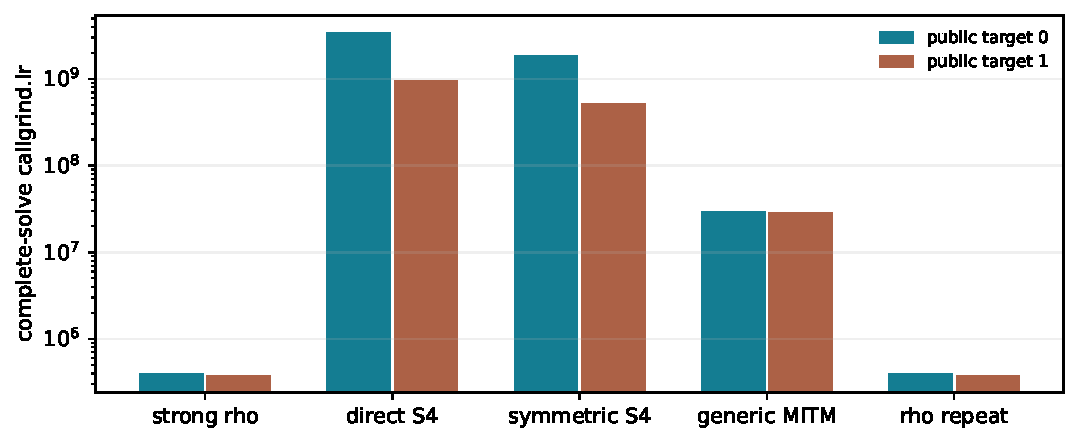
\includegraphics[width=.98\linewidth]{complete-solve-ir.pdf}\end{center}
\begin{center}\begin{tabular}{rlrr}\toprule
Seq & arm & whole-solve Ir & Ir / same-target rho\\\midrule
0 & rho-strong & 394,957 & 1 \\
1 & ic-direct & 3,437,956,039 & 8704.63 \\
2 & ic-symmetric & 1,886,477,140 & 4776.41 \\
3 & ic-pair-table & 29,809,413 & 75.4751 \\
4 & rho-strong-aa & 394,957 & 1 \\
5 & rho-strong & 382,326 & 1 \\
6 & ic-direct & 969,572,722 & 2535.98 \\
7 & ic-symmetric & 519,382,510 & 1358.48 \\
8 & ic-pair-table & 28,583,994 & 74.7634 \\
9 & rho-strong-aa & 382,326 & 1 \\
\bottomrule\end{tabular}\end{center}

All ten recovered scalars independently reproduce the recorded target by
generator multiplication. Every integer phase counter, native counter,
factor-base record and solver-word count matches the native run. Four rho
rows have a one-ULP serialized phase-price difference; the strict failed
check is retained, numerical prices use the explicit 1e-12 relative tolerance,
and per-row exactness flags remain visible. Six IC rows have bit-exact prices.
The final native audit reproduces byte for byte, including per-marker sums.

The native parser recovers a complete-solve interval for all ten profiles.
The four rho profiles also have target-only boundaries; the six IC profiles
do not. Their online intervals remain null, with exact parser refusals.
No IC online speed comparison is inferred. Per-marker attribution is in the
native receipt; the PDP marker contains construction, solving and splitting
together and does not separately price those operations.

Valgrind 3.24.0, one thread, local AMD EPYC 9V74 host, L0, 360 seconds per
child. These are user-space implementation instruction counts under the
Valgrind allocator. Native allocator work is absent; profile wall times are
diagnostics. No PMU or GPU is exposed. Ir ratios are not runtime speedups,
hardware calibration or complete GAE prices. No algorithmic improvement,
fastest-tool claim or leaderboard promotion is made from this profile.

Protocol: \path{../../PROFILE_PROTOCOL.md}. Native validator:
\path{examples/ic_instruction_profile_audit.rs}.
Receipt: \path{../../pipeline-receipts/instruction-profiles-n13-20261025-01/receipt.json}.
Raw archive under evidence/: \path{runs-instruction-profiles-n13-20261025-01.tar.xz}.
Publication of oversized artifacts remains blocked; unchanged bytes are local.

\end{document}
